\section{Задание 2. Кривые второго порядка.}

\textbf{Условие.}

Даны уравнения двух множеств:

Множество 1: $40x^2 + 36xy + 25y^2 - 8x - 14y + 1 = 0$

Множество 2: $5x^2 + 4xy - y^2 - 5x + y = 0$

\begin{enumerate}
    \item Покажите, что одно из множеств является кривой второго порядка, сведя его
    уравнение к каноническому виду преобразованием координат, а другое – кривой,
    распавшейся на прямые (найдите уравнения прямых).
    \item Изобразите каждое множество на отдельном рисунке вместе со старой и новой
    системой координат (оси новой системы должны служить осями симметрии
    множества).
    \item У нераспавшейся кривой определите расстояние $p$ между фокусом и директрисой и
    эксцентриситет $\varepsilon$. Запишите полярное уравнение кривой с найденными параметрами.
    \item На одном рисунке совместите началами и осями $Ox$ декартову прямоугольную и
    полярную системы координат. Постройте кривую по ее каноническому уравнению в
    ДПСК и по ее полярному уравнению в ПСК. Объясните несовпадение кривых.
    \item Найдите такое расположение ПСК и формулы преобразования полярных координат в
    декартовы, чтобы полярное и каноническое уравнения описывали одну и ту же
    кривую.
\end{enumerate}
\vspace{10mm}
\textbf{Решение.}
\begin{enumerate}
    \linespread{3}
    \item Сгруппируем второе уравнение: $5x^2 + 4xy - y^2 -5x + y = -x(y - 5x) - y(y - 5x) + (y - 5x) = (1 - x - y)(y - 5x) = 0$. Из этого мы видим, что это уравнение описывает две прямые
    $1 - x - y = 0$ и $y - 5x = 0$.

    \item Избавимся от части первого уравнения с $xy$ с помощью поворота СК: $40x^2 + 36xy + 25y^2 - 8x - 14y + 1 \Rightarrow $ нужно повернуть СК на угол $\alpha,  \tg(2\alpha) = \frac{36}{40 - 25} = \frac{12}{5}$.

    Тогда:
    \(\cos(2\alpha) = \frac{5}{13} \Rightarrow 2\cos^2(\alpha) - 1 = \frac{5}{13} \Rightarrow \cos^2(\alpha) = \frac{9}{13} \Rightarrow \cos(\alpha) = \frac{3\sqrt{13}}{13} \Rightarrow \sin(\alpha) = \frac{2\sqrt{13}}{13}\)

    Новые координаты: $ \displaystyle
    \begin{cases}
        x' = x\cos(\alpha) - y\sin(\alpha) \\
        y' = x\sin(\alpha) + y\cos(\alpha)
    \end{cases} \Rightarrow
    \begin{cases}
        x' = \frac{3x\sqrt{13}}{13} - \frac{2y\sqrt{13}}{13}\\
        y' = \frac{2x\sqrt{13}}{13} +\frac{3y\sqrt{13}}{13}
    \end{cases} \Rightarrow \\
    40x^2 + 36xy + 25y^2 - 8x - 14y + 1 = 0 \Rightarrow \\
    40\left(\frac{3x'\sqrt{13}-2y'\sqrt{13}}{13}\right)^{2}+36\left(\frac{\left(3x'\sqrt{13}-2y'\sqrt{13}\right)\left(3y'\sqrt{13}+2x'\sqrt{13}\right)}{169}\right)+25\left(\frac{3y'\sqrt{13}+2x'\sqrt{13}}{13}\right)^{2}\ -8\left(\frac{3x'\sqrt{13}-2y'\sqrt{13}}{13}\right)-14\left(\frac{3y'\sqrt{13}+2x'\sqrt{13}}{13}\right)+1=
    52x'^2+13y'^2- 4x'\sqrt{13}-2y'\sqrt{13} + 1 = \left(2x'\sqrt{13} - 1\right)^2 + (y'\sqrt{13} - 1)^2 - 1 = 0 \Rightarrow \\
    \frac{\left(x' - 1/2\sqrt{13}\right)^2}{1/52} + \frac{\left(y' - 1/\sqrt{13}\right)^2}{1/13} = 1 $
    \item Тогда сместим начало координат на $(\frac{1}{2\sqrt{13}}; \frac{1}{\sqrt{13}}) \Rightarrow $
    $\begin{cases}
         x'' = x' - \frac{1}{2\sqrt{13}}\\ y'' = y' - \frac{1}{\sqrt{13}}
    \end{cases} \Rightarrow \frac{x''^2}{1/52} + \frac{y''^2}{1/13} = 1$ - получили вертикально ориентированный эллипс.

    Для удобства сделаем его горизонтально ориентированным: $\frac{x''^2}{1/13} + \frac{y''^2}{1/52} = 1$ - каноническое уравнение кривой 2 порядка.
    \item Изображения кривой в старой и новой системе координат:
    \begin{figure}[H]
        \centering
        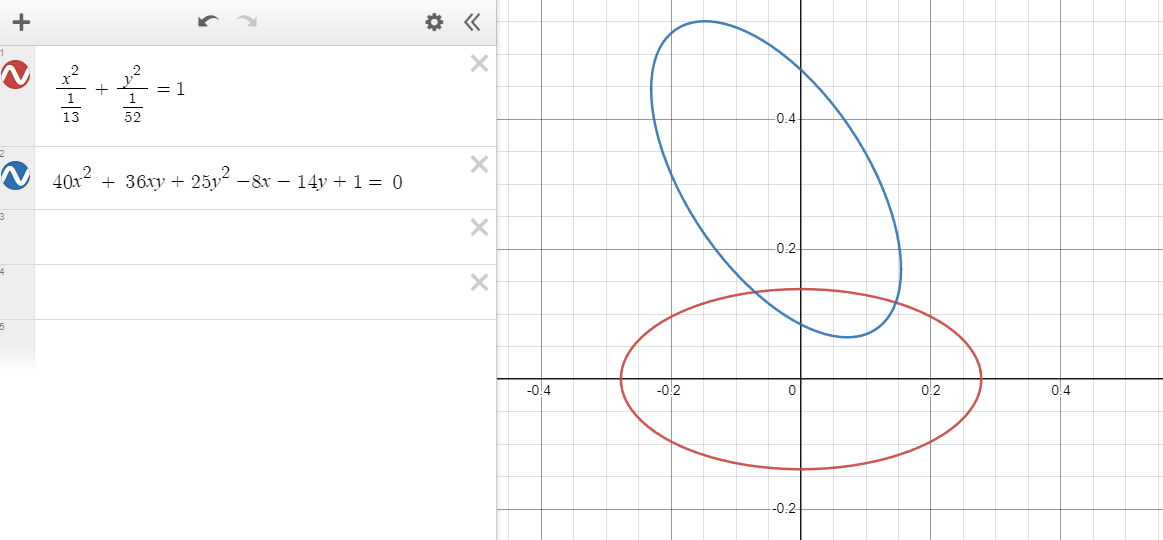
\includegraphics[width=1\linewidth]{images/2_b_1}
    \end{figure}
    \begin{figure}[H]
        \centering
        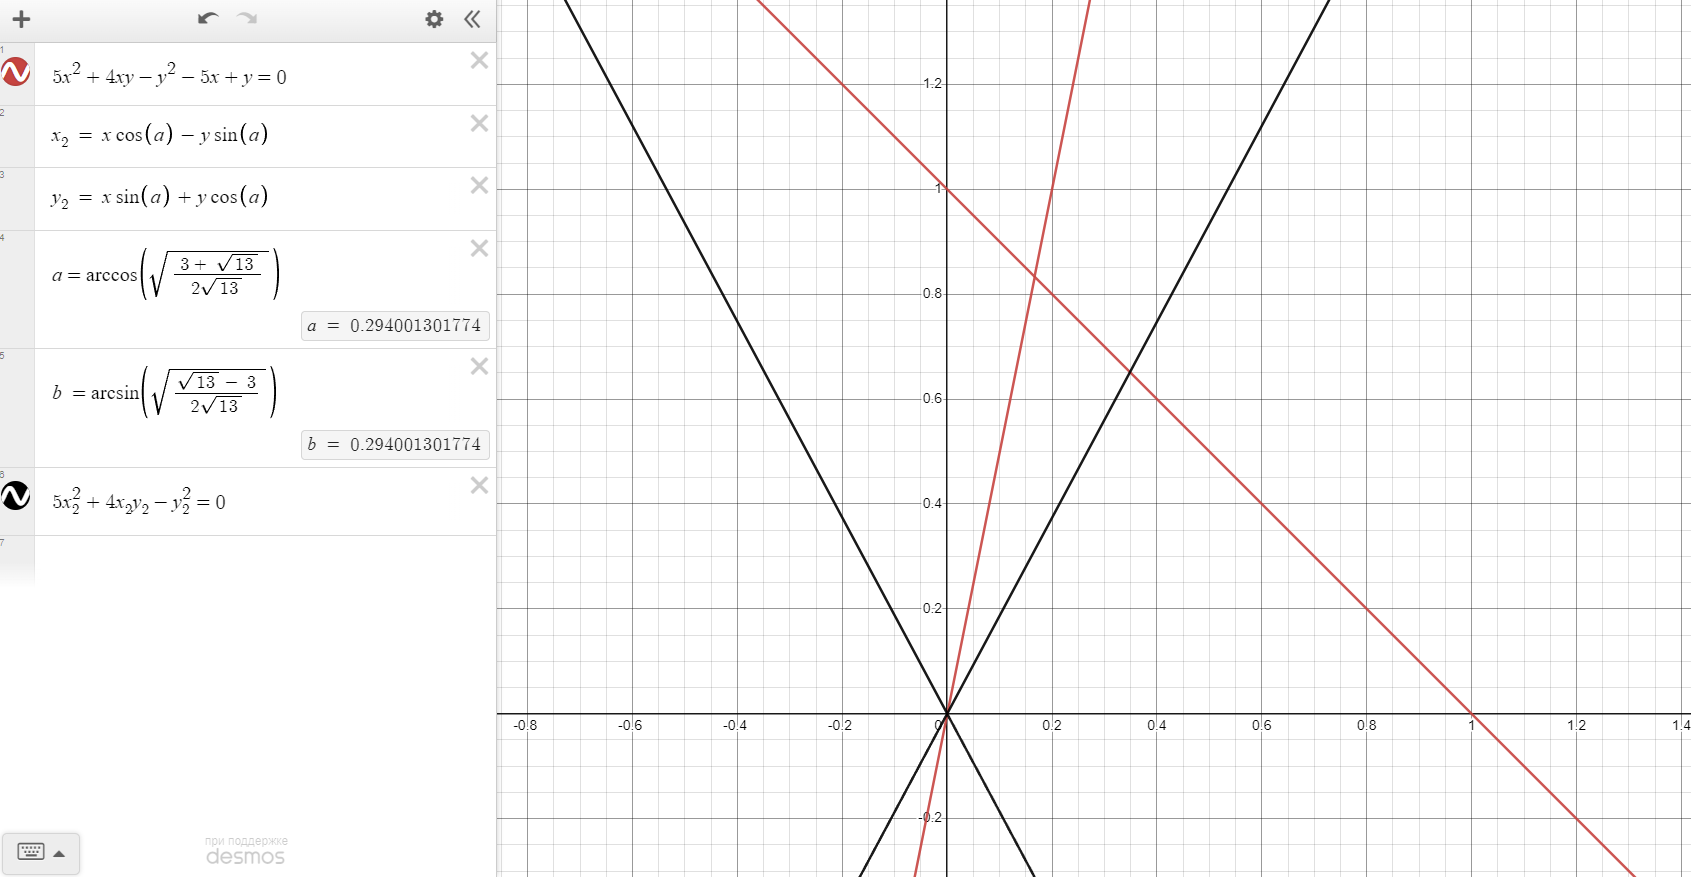
\includegraphics[width=1\linewidth]{images/2_b_2}
    \end{figure}

    \item Из уравнения $\frac{x^2}{1/13} + \frac{y^2}{1/52} = 1$ находим $c = \sqrt{a^2 - b^2} = \sqrt{\frac{3}{52}} \Rightarrow \epsilon = \frac{c}{a} = \frac{\sqrt{3}\sqrt{13}}{\sqrt{52}} = \frac{\sqrt{3}}{2} \Rightarrow d: x = \pm\frac{a}{\epsilon} = \frac{2}{\sqrt{3}\sqrt{13}}, F = (\pm c; 0) \Rightarrow p =  \mid c - \frac{a}{\epsilon} \mid  =  \mid \frac{\sqrt{3}}{2\sqrt{13}} - \frac{2}{\sqrt{3}\sqrt{13}} \mid  =  \mid \frac{3 - 4}{2\sqrt{3}\sqrt{13}} \mid  =  \frac{1}{2\sqrt{39}}$.\\

    Полярное уравнение кривой в таком случае: $r = \frac{\frac{1}{4\sqrt{13}}}{1 - \frac{\sqrt{3}}{2}\cos(\phi)} = \frac{1}{4\sqrt{13} - 2\sqrt{39}\cos(\phi)}$

    \item Кривые не совпадают, так как в ПСК начало координат оказывается в фокусе эллипса, а в ДПСК в центре эллипса.
    \begin{figure}[H]
        \centering
        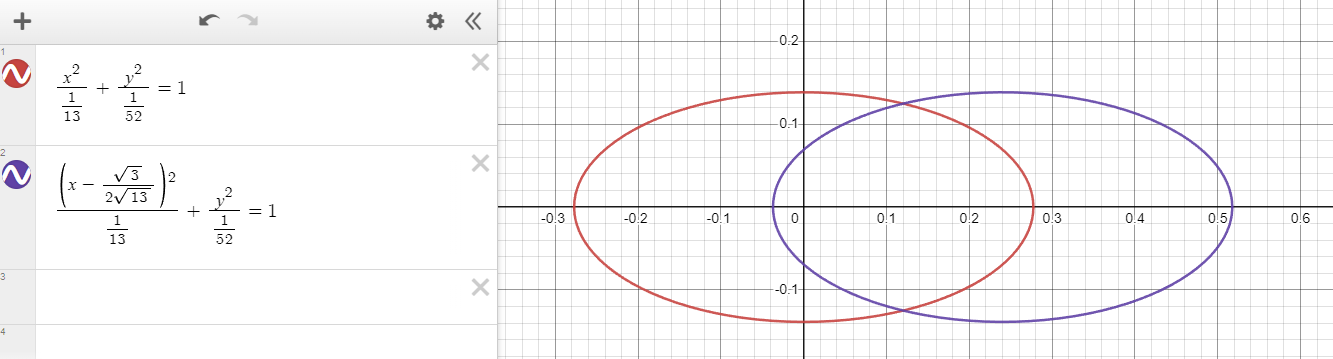
\includegraphics[width=1\linewidth]{images/2_c_1}
    \end{figure}

    \item Начало координат в ПСК должно быть смещено на $(-c; 0)$ относительно начала координат в ДПСК. Преобразуем формулы перехода из ПСК в ДПСК: $\begin{cases}
                                                                                                                                                         x = r\cos(\phi)\\ y = r\sin(\phi)
    \end{cases} \Rightarrow
    \begin{cases}
        x' =  x - c \\ y' = y
    \end{cases} \Rightarrow
    \begin{cases}
        x' = r\cos(\phi) - \frac{\sqrt{3}}{2\sqrt{13}}\\ y'  = r\sin(\phi)
    \end{cases}$

\end{enumerate}

\clearpage